\documentclass[runningheads]{llncs}
\usepackage{fontspec}
\setmainfont{Times New Roman}
\usepackage{amsmath,amssymb,graphicx,booktabs,url,array}
\setlength{\emergencystretch}{3em}
\renewcommand{\abstractname}{Özet.}
\renewcommand{\keywordname}{\textbf{Anahtar sözcükler:}}
\renewcommand{\figurename}{Şekil}
\renewcommand{\tablename}{Tablo}
\renewcommand{\refname}{Kaynakça}
\title{Sıfır Entropi Kabul Kanıtı Değildir:\\Gereksinim Kararlarında Temsil ve Kanıtın Ayrılması}
\titlerunning{Gereksinim Kararlarında Temsil ve Kanıt}
\author{ChatGPT}
\authorrunning{ChatGPT; yönlendiren Volkan Aran}
\institute{Yönlendiren: Volkan Aran\\Araştırma notu; yazar atıflı çalışma nüshası}
\begin{document}
\maketitle
\begin{abstract}
Gereksinimlerin ayrıntılandırılmasında seçeneklerin azalması, uygulamanın gereksinimi karşıladığını göstermez. Bu çalışma, entropiye dayalı tamamlanma göstergelerinin iki sınırını inceler: aynı kanıt altında etiket sayısı değişince entropi değişebilir; aynı entropi altında kabul sonucu değişebilir. İlk sınır Shannon entropisinin ayrıştırma özelliğiyle, ikincisi eş entropili karşı örnekle gösterilir. Bu ayrımdan küçük bir kayıt sözleşmesi türetilir: kararın kapanması, önceden belirtilmiş tasarım sınıflarının pozitif destek sayısına; kabul ise kapsamı, sürümü ve uygulaması eşleşen test kayıtlarına bağlıdır. Python uygulaması 2.480 sonlu durum, 7.440 dönüşüm kontrolü, 52 sayısal sınır ve 41 geçersiz kayıt üzerinde sınanmıştır. MATLAB, toplam 2.573 temel kaydın durumlarını yeniden hesaplamıştır. RFC~9110'dan alınan iki HEAD koşulu için dört kontrollü sunucu çeşidine 40 gerçek yerel HTTP isteği gönderilmiştir. Dördünde de karar entropisi sıfırken iki çeşidin testleri başarısız olmuştur. Katkı, yeni bir entropi kuramı veya sistem doğruluğu ispatı değil; temsil değişimini kanıttan ayıran, açık varsayımlara sahip ve çalıştırılabilir bir yöntem sınırıdır.
\keywords{Gereksinim mühendisliği \and Entropi \and Temsil değişmezliği \and Kabul kanıtı}
\end{abstract}

\section{Problem ve Katkının Sınırı}
Bir projenin sonunda tek tasarım seçilmiş olabilir; seçilen tasarım yine de hatalı olabilir. Tersine, bir uygulama testleri geçerken başka uygun tasarımlar açık kalabilir. Dolayısıyla ``ne yapacağımıza karar verdik'' ile ``yaptığımızın ölçütleri karşıladığına dair kayıt var'' farklı önermelerdir. Bu makalenin savı şudur: \emph{bir temsilin düzenlenmesiyle elde edilen kesinlik, davranışa ilişkin gerekçenin yerine geçemez.}

Bu ayrım gereksinim mühendisliği için yeni değildir. Zave ve Jackson~\cite{zave}, biçimsel ifadelerin anlamının çevredeki olgulara bağlanmasını ve gereksinimlerin alan bilgisiyle ilişkilendirilmesini vurgular. Gereksinim kalitesi araştırması da bir çalışma ürünü özelliğinin pratik etkisiyle ilişkisinin ayrıca açıklanmasını gerektirir~\cite{quality}. SACM~\cite{sacm}, iddia, gerekçe ve kanıt için daha geniş bir model sunar. Burada bu yaklaşımların yerine geçecek bir güvence sistemi önerilmemektedir. Daha dar problem, \emph{bir belirsizlik göstergesinin hangi dönüşümler altında karar ve kabul bilgisini koruduğudur}.

Çalışmanın ilk kurgusu, tek satırdan büyüyen siyah-beyaz hücresel otomat görüntüsünü gereksinim ayrıntılandırmasına benzetiyordu. Wolfram'ın hesaplamaya ve gözlemciye bağlı betimlemeler tartışması~\cite{wolfram} bu kurgunun esin kaynağıdır. Ancak benzetme, yazılım projesine bir termodinamik yasa sağlamaz. Hücre kurallarıyla görüntüyü silmek veya beyaz alan eklemek test kanıtı üretmez. Bu nedenle burada hücresel otomatın yararlılığı, düşünme sürecini temsil ettiği ve projenin sonunda toplam belirsizliğin sıfırlandığı iddiaları çıkarılmıştır.

Katkı üç parçadır: (1) etiket entropisi ile kabul arasında iki açık sınır önermesi; (2) bu sınırları koruyan sınıf, destek ve kanıt sözleşmesi; (3) sonlu kontroller ve dış kaynaklı bir şartnameye bağlı çalıştırılmış örnek. Sonuçlar, insanların daha iyi karar verdiği veya endüstriyel proje başarısının arttığı iddiasını taşımaz. Araştırma sorusu, bu sınırlı sözleşmenin temsil değişikliği ve sayısal sınırlar altında tutarlı uygulanıp uygulanamadığıdır.

\section{Model: Neyin Belirsizliği, Neyin Kabulü?}
Bir kayıt; gereksinim kimliği $r$, kapsam/sürüm kimliği $v$, uygulama kimliği $i$, gerekli ölçütler kümesi $C$, aday etiketleri $A$, kanıt kayıtları $E$ ve iki açık bildirim içerir: ölçüt kapsamının incelendiği $d$ ve karar çelişkisi bulunduğu $z$. Bu bildirimler dış girdidir; yazılım bunların gerçekliğini çıkarmaz.

Her $a\in A$ için negatif olmayan ağırlık $w_a$ ve bir sınıf kimliği $\gamma(a)$ verilir. Sınıf, bu kaydın karar kapsamı içinde aynı tasarımı belirten etiketleri birleştirir. Örneğin aynı kod sürümünün iki adı tek sınıftır. \emph{Aynı testleri geçmek, farklı tasarımları otomatik olarak eşdeğer yapmaz.} Sınıf eşlemesi sabit tutulur; değişmesi yeni bir modelleme kararıdır ve gerekçe gerektirir. Doğal dilden eşdeğerlik çıkarımı kapsam dışıdır.

Normalize ağırlık ve sınıf ağırlığı şöyle tanımlanır:
\begin{equation}
p_a=\frac{w_a}{\sum_b w_b},\qquad P_g=\sum_{a:\gamma(a)=g}p_a.
\end{equation}
Bunlar modelde verilmiş ağırlıklardır; testlerle kalibre edilmiş doğruluk olasılıkları değildir. İki ayrı entropi ve bir destek sayısı hesaplanır:
\begin{equation}
H_A=-\sum_{p_a>0}p_a\log_2p_a,\quad
H_G=-\sum_{P_g>0}P_g\log_2P_g,\quad
S=|\{g:P_g>0\}|.
\end{equation}
Karar, $z=0$ ve $S=1$ olduğunda kapalıdır; $z=0$, $S>1$ iken açıktır; $z=1$ iken tutarsızdır. Ağırlığı sıfır olan adaylar elenmiş sayılır. Bu, kayda alınmamış seçeneklerin bulunmadığını söylemez.

Her kanıt; kendi kimliğini, ölçüt kimliğini, $(r,v,i)$ bağını, kaynak ve değerlendirici kimliğini, onay işaretini ve geçti/kaldı sonucunu taşır. $B$; her gerekli ölçütün tam bir kez kapsandığını, bağların eşleştiğini ve onayların bulunduğunu göstersin. Geçerli kayıtlar için kabul politikası:
\begin{equation}
K=\begin{cases}
\text{beklemede},&\neg d\;\lor\;z\;\lor\;\neg B,\\
\text{başarısız},&d\land\neg z\land B\land\exists e:\operatorname{sonuç}(e)=\text{kaldı},\\
\text{kayıtlara göre kabul},&d\land\neg z\land B\land\forall e:\operatorname{sonuç}(e)=\text{geçti}.
\end{cases}
\end{equation}
Öncelik bilinçlidir: eksik kapsam altında bazı başarısız testler bulunsa bile genel durum beklemededir; ham başarısız sonuçlar kaybolmaz. Bu politika, her ölçüt için tek bir değerlendirilmiş kayıt ister. Çoklu deneme ve çelişen kanıtları birleştirme ayrı bir problemdir.

\section{İki Sınır Önermesi ve Bir Tasarım İlkesi}
\subsection{Aynı kanıt, farklı entropi}
\textbf{Önerme 1 (etiket ayrıştırması).} Ağırlığı $p_a$ olan bir etiket aynı sınıfta $q_1,\ldots,q_m$ oranlarıyla bölünsün; $q_j\geq0$, $\sum_jq_j=1$ olsun. Diğer sınıflar, kapsam ve kanıt değişmesin. O zaman
\begin{equation}
H'_A-H_A=p_aH(q),\qquad H'_G=H_G,\quad S'=S,\quad K'=K.
\end{equation}
\textit{Gerekçe.} Yeni etiketlerin katkısı $-\sum_jp_aq_j\log_2(p_aq_j)$ ifadesidir. Açıldığında eski katkı ve $p_aH(q)$ elde edilir. Sınıf toplamı aynı kaldığı için diğer eşitlikler korunur. Bu, Shannon'ın ayrıştırma özelliğinin~\cite{shannon} doğrudan uygulamasıdır; yeni bir bilgi kuramı sonucu değildir.

Örneğin tek tasarıma iki eşit etiket verilmesi $H_A$ değerini 0'dan 1 bite çıkarır. Yeni tasarım veya test oluşmadığından $H_G=0$ ve kabul değişmez. Eşdeğerlik ilişkisi yanlış kurulursa sınıf entropisi de yanlış yoruma açıktır. Sınıflandırma anlamsal yükü ortadan kaldırmaz; nerede taşındığını görünür kılar.

\subsection{Aynı entropi, farklı kabul}
\textbf{Önerme 2 (entropinin tek başına yetersizliği).} Aynı aday dağılımını koruyup güncel test sonucunu geçti ile kaldı arasında değiştirmeye izin veren kayıt alanında, tüm kayıtların kabulünü doğru veren yalnızca $H_A$ veya $H_G$ değerine bağlı bir fonksiyon yoktur.

\textit{Gerekçe.} $d=1,z=0,S=1$ olan iki geçerli kayıt seçilsin. Ölçütler ve bağlar tam olsun. Birincide bütün sonuçlar geçti, ikincide en az biri kaldı olsun. İkisinde de $H_A=H_G=0$ olabilir; kabul sonuçları farklıdır. Aynı girdiye iki farklı çıktı veremeyeceği için böyle bir fonksiyon yoktur. Dağılımın tamamını girdi alan bir fonksiyon da bu örnek çiftini ayıramaz.

Önerme, kanıttan bağımsız dağılım tutulan bu model alanına aittir. Kanıtı özel olarak kodlayan bir dağılımın farklı varsayımlar altında yararlı olamayacağını söylemez. Kanıt ile seçimi ayırmak genel olarak bilinen bir gerekliliktir; buradaki yararı, entropiye dayalı kapanma iddiasının tam olarak hangi varsayımda başarısız olduğunu belirlemesidir.

\subsection{Sayısal sıfır yerine yapısal kapanma}
Kesin aritmetikte $H_G=0$ ile $S=1$ eşdeğerdir. Ancak $H_G\leq\varepsilon$ testi aynı şey değildir. $p=(1-2^{-k},2^{-k})$ için her sonlu $k$ değerinde iki aday pozitiftir; entropi sıfıra yaklaşır. Bu nedenle kapanma, kayan noktalı entropi karşılaştırmasından değil pozitif sınıf ağırlıklarının sayısından hesaplanır. Gösterim, durum hesabıyla aynı \texttt{closed} alanını kullanmalıdır. Entropinin ekranda yuvarlanarak 0 görünmesi, durum etiketini değiştirmez.

\begin{figure}[t]
\centering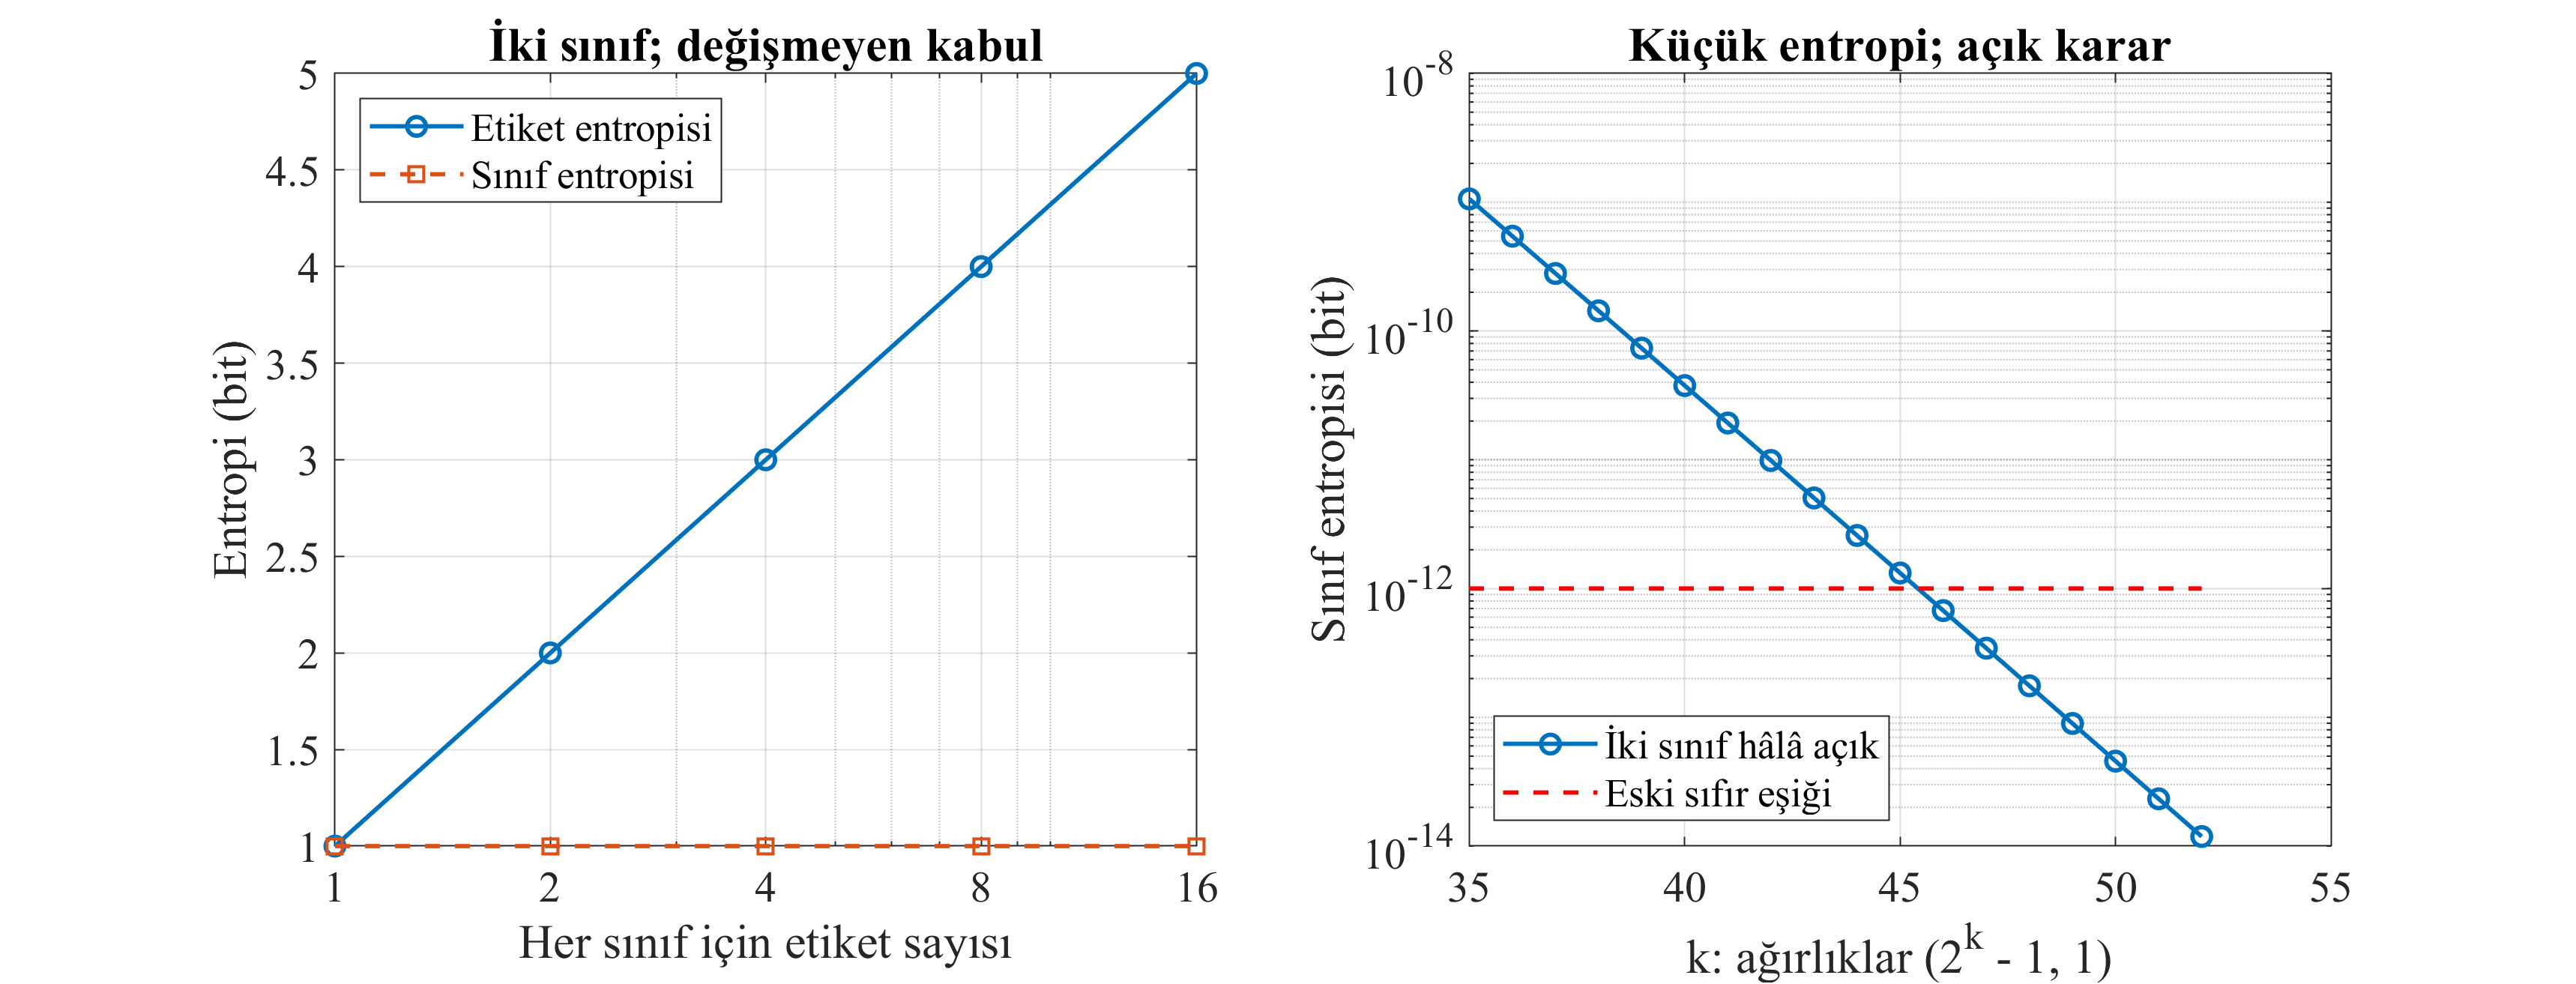
\includegraphics[width=\textwidth]{assets/ayrimlar.png}
\caption{MATLAB ile yeniden hesaplanan iki kontrol. Solda her birinin ağırlığı $1/2$ olan iki tasarım sınıfı, sınıf başına 1--16 eşit etiketle gösterilir; $H_G=1$ değişmezken $H_A$ artar. Sağda iki pozitif sınıf korunmasına rağmen entropi eski $10^{-12}$ eşiğinin altına iner. Hiçbir eğri uygulama doğruluğunu ölçmez.}\label{fig:limits}
\end{figure}

\section{Çalıştırılabilir Sözleşme ve Yeni Kontroller}
\subsection{Uygulama kararları}
Python ve MATLAB uygulamaları aynı sınırlı şemayı ayrı kodlarla değerlendirir. Bütün kimlikler metin olmalı, boş olmamalı ve başta/sonda boşluk taşımamalıdır. Aday, ölçüt ve kanıt kimliklerinin gerekli tekillikleri denetlenir; bilinmeyen ölçüt veya yinelenen kapsam geçersizdir. Bu koşullar artık varsayılan belge kuralları değildir; çalıştırılan denetimlerdir.

Kayan noktalı ağırlıkların sıfıra yuvarlanmasını önlemek için çalıştırılabilir şema, toplamı $1\leq W\leq2^{52}$ olan tamsayı ağırlıkları kullanır. Böylece MATLAB'ın double gösteriminde tamsayılar tam temsil edilir; destek hesaplanırken normalizasyon yapılmaz. Entropi yalnızca raporlanan yaklaşık sayıdır. Bu kısıt keyfi gerçek olasılıkları kapsamaz; önceki serbest ağırlık arayüzüne göre bilinçli bir kapsam daraltmasıdır. Karar çelişkisi veya geçersiz girdi, kapanmış durum üretmez.

Kaynak ve değerlendirici kimlikleri birer bildirimdir; dolu olmaları doğruluklarını ispatlamaz. Kayıt denetleyicisi test dosyasını yeniden çalıştırmaz veya dış veriyi doğrulamaz. HTTP örneğindeki ayrı deney sürücüsü gerçek yanıtları kaydeder ve ölçüt sonucunu üretir; denetleyici bu sonucu tüketir. Bu görev ayrımı, kanıt üretimi ile kayıt tutarlılığını karıştırmayı önler.

\subsection{Sonlu alan ve dönüşüm kontrolleri}
Temel alan, $n=1,2,3$ ölçüt için her ölçüte beş durum atar: geçti, kaldı, eksik, eski sürüm ve başka uygulama. İki inceleme işareti, iki çelişki işareti ve dört aday profili çaprazlanır. Profiller tek pozitif sınıf, eşit iki sınıf, çok dengesiz iki sınıf ve aynı sınıfa ait iki etikettir. Toplam
\begin{equation}
(5+5^2+5^3)\times2\times2\times4=2.480
\end{equation}
kayıt oluşur. Beklenen kabul, üreticinin atadığı kanıt durumlarından; beklenen karar, profilin sınıflarından türetilir. Bu, anlamsal doğruluğun bağımsız hakem testi değil, belirtilen sözleşmeyle uygulama uyumunun kontrolüdür.

Her kayıt için üç dönüşüm daha sınanır: (i) bütün aday etiketlerini aynı sınıfta ikiye bölme, (ii) aday sırasını ters çevirme, (iii) kanıtı yenilemeden sürümü değiştirme. İlkinde sınıf entropisi ve durumlar korunmalı, etiket entropisi 1 bit artmalıdır; ikincide tüm sonuçlar aynı kalmalıdır; üçüncüde kabul verilmemelidir. Toplam 7.440 kontrol bu ilişkileri sağlamıştır.

\begin{table}[t]
\caption{Yeni çalıştırmanın kapsamı. Sayılar bağımsız proje veya insan sayısı değildir.}\label{tab:tests}
\centering\small\setlength{\tabcolsep}{4pt}
\begin{tabular}{p{.32\textwidth}r p{.48\textwidth}}
\toprule Kontrol & Sayı & Gözlenen sonuç\\\midrule
Temel durum çaprazlaması & 2.480 & 12 kabul, 44 başarısız, 2.424 beklemede; beklentiyle tam eşleşme\\
Dönüşüm ilişkileri & 7.440 & İhlal yok; entropi ilişkilerinde Python farkı 0\\
$k=1,\ldots,52$ sınırları & 52 & Hepsi açık; eski eşik 7'sini kapatırdı\\
Geçersiz kimlik/ağırlık & 41 & Hepsi geçersiz; kabul üretilmedi\\
MATLAB yeniden hesabı & 2.573 & Durumlar aynı; azami entropi farkı \mbox{$6{,}94\times10^{-18}$}\\
Yerel HTTP istekleri & 40 & 20 GET/HEAD çifti; dört kontrollü çeşitten ikisi başarısız\\\bottomrule
\end{tabular}
\end{table}

Sınır taramasında $k=46,\ldots,52$ için eski $10^{-12}$ kuralı yanlış kapanma verirken destek kontrolü kararı açık tutmuştur. Örneğin $k=50$ için $H_G\approx4{,}57\times10^{-14}$ bittir, fakat $S=2$'dir. MATLAB, 2.480 temel, 52 sınır ve 41 geçersiz kaydı okuyarak kendi denetleyicisiyle değerlendirmiştir. Bu hesaplar test kapsamı içinde kod uyumunu gösterir; ispatların veya alan uzmanı incelemesinin yerine geçmez.

\section{Dış Kaynaklı Gereksinimle Çalıştırılmış Örnek}
\subsection{Şartnameden ölçüte}
RFC~9110~\cite{rfc}, HEAD yanıtında içerik gönderilmemesini ister (Bölüm~9.3.2). Content-Length alanı varsa aynı GET isteğinin içerik uzunluğunu göstermelidir (Bölüm~8.6). Daraltılmış gereksinimimiz, sabit bir kaynağın başarılı HTTP/1.1 yanıtında bu iki koşulun sağlanmasıdır. Ölçütler $C_1$: HEAD içerik baytı sayısı sıfır; $C_2$: Content-Length yok veya gözlenen GET uzunluğuna eşit olarak kodlanmıştır. Alanın bulunmaması başarısızlık değildir.

Yerel TCP sunucusunun dört kontrollü çeşidi çalıştırılmıştır: doğru uzunluk bildiren, HEAD'de uzunluk alanını atlayan, yasak içerik gönderen ve uzunluğu yanlışlıkla sıfır bildiren. Her çeşide 0, 1, 7, 64 ve 1.024 baytlık sabit kaynaklar için birer GET/HEAD çifti gönderilmiştir. Test istemcisi ham soket baytlarını kaydeder; HEAD içeriğini gizleyebilen üst düzey istemci davranışına dayanmaz. Bağlantı yanıt sonunda kapanır; aktarım kodlaması, sıkıştırma, eşzamanlı değişim ve ara sunucu yoktur. GET içeriğinin beklenen kaynağa eşitliği ayrıca denetlenir.

\begin{table}[t]
\caption{Her çeşitte tek seçilmiş tasarım ($H_G=0$). Ölçüt sonucu beş kaynak üzerinde birleşiktir.}\label{tab:http}
\centering\small\setlength{\tabcolsep}{4pt}
\begin{tabular}{p{.34\textwidth}ccp{.30\textwidth}}
\toprule Çeşit & $C_1$ & $C_2$ & Kayıt sonucu\\\midrule
Doğru uzunluk & Geçti & Geçti & Kapsam içinde kabul\\
Uzunluk alanı yok & Geçti & Geçti & Kapsam içinde kabul\\
HEAD içeriği var & Kaldı & Geçti & Başarısız\\
HEAD uzunluğu sıfır & Geçti & Kaldı & Başarısız\\\bottomrule
\end{tabular}
\end{table}

İki hatalı çeşit boş kaynakta ayırt edilmez, dört boş olmayan kaynakta ilgili ölçütü ihlal eder. Her ölçüt için beş sonucun birleşimi tek kanıt kaydına dönüştürülmüştür. Ölçüt kapsamının inceleme işareti deney protokolünün beyanıdır; bağımsız insan onayı yapılmamıştır. Burada gerçek ağ üstünden ölçülmüş yazılım davranışı vardır; sunucular ve hatalar araştırma için oluşturulmuştur. Dolayısıyla bu bir endüstriyel vaka veya tüm HTTP uyumluluğu testi değildir.

\subsection{Altı aşamalı proje kaydı}
Tablo~\ref{tab:flow}, aynı deneyin karar ve kanıtlarını altı olayla özetler. Seviyeler zorunlu süreç basamakları değil, kaydın ardışık anlarıdır. İlk iki aşamada test yoktur. Üçüncü aşamadaki başarısız kanıt, uygulama değiştirilince yeni uygulamanın kanıtı olmaz. Beşinci aşamadaki yeni testlerden sonra kabul verilebilir. Son aşamadaki iki ad aynı kodu işaret ettiğinden yalnızca etiket entropisi artar.

\begin{table}[t]
\caption{Karar kapanması ve kabul aynı anda, tek yönde ilerlemek zorunda değildir.}\label{tab:flow}
\centering\small\setlength{\tabcolsep}{4pt}
\begin{tabular}{cp{.43\textwidth}ccp{.22\textwidth}}
\toprule Seviye & Olay & $H_A$ & $H_G$ & Kabul\\\midrule
1 & İki tasarım; test yok & 1 & 1 & Beklemede\\
2 & Tek tasarım seçildi & 0 & 0 & Beklemede\\
3 & Test hatayı gösterdi & 0 & 0 & Başarısız\\
4 & Kod düzeltildi; kanıt eski & 0 & 0 & Beklemede\\
5 & Yeni sürümün testleri geçti & 0 & 0 & Kabul\\
6 & Aynı koda iki eşit etiket & 1 & 0 & Kabul\\\bottomrule
\end{tabular}
\end{table}

Bu örnekte doğru uzunluk bildiren ve uzunluk alanını atlayan kodlar farklı tasarım sınıflarıdır. Her ikisi ölçütleri sağlayabilir. Bu iki sınıf açık bırakıldığında da test edilen belirli uygulamanın kabulü sürer. Böylece sıfır entropinin ne yeterli ne de bu politika altında gerekli olduğu somutlaşır.

\section{Tartışma, Sınırlılıklar ve Sonuç}
\textbf{Felsefi sonuç.} Entropi, önce neyin ayrı seçenek sayıldığına ilişkin bir karar ister. Bu karar salt sayısal değildir: aynı koda verilen iki ad ile iki farklı kodu ayırmak için yorum gerekir. Model, bu yorumu sınıf eşlemesine; davranış iddiasını ölçüt ve kanıta; aritmetiği entropi hesabına yerleştirir. Bir hesabın doğru olması, hesabın dünyaya doğru bağlandığı anlamına gelmez. Çalışmanın gücü, bu bağı otomatik kurduğunu iddia etmek yerine kontrol edilebilir sınırlarını göstermesidir.

\textbf{Yakın yaklaşımlarla ilişki.} Shannon'ın ayrıştırma özelliği matematiksel temeli zaten verir; bu makale o özelliği yeni teorem olarak sunmaz. Zave--Jackson'ın anlam ile biçim ayrımı gereksinim düzeyindeki temeldir. SACM, gerekçe ve kanıtın daha kapsamlı örgütlenmesini sağlar; burada bunun yerine yalnızca bir kayıt kabul koşulu uygulanır. Bu çalışmaya özgü birleştirme, etiket/sınıf ayrımını, kesin destekle kapanmayı ve sürüme bağlı kabulü aynı küçük deneyde sınamaktır. Bu yaklaşımlara performans veya doğruluk üstünlüğü ölçülmemiştir.

\textbf{Geçerlilik sınırları.} Eşdeğerlik sınıfları, ağırlıklar ve ölçütler dışarıdan belirlenir. Yanlış ölçüt, eksik aday kümesi veya sahte kanıt, biçimsel kontrollerden geçebilir. İki dilde aynı sonucun alınması ortak kavramsal hatayı dışlamaz. Sonlu tarama bütün girdileri veya programın tam doğruluğunu ispatlamaz. HTTP örneği iki koşul ve beş kaynakla sınırlıdır. Test edilen sunucu kodu ve ölçüt kodu aynı çalışma içinde yazılmıştır; bağımsız değerlendirme yoktur. Kullanıcı yararı, doğal dil çözümleme ve termodinamik açıklama için veri üretilmemiştir.

\textbf{Sonuç.} Entropinin sıfırlanması, tanımlı seçenek uzayında seçimin kapanması olarak yorumlanabilir; kabul için ayrıca kapsamı ve uygulaması belli kanıt gerekir. Etiket ayrıştırması altında korunması gereken değişken sınıf dağılımıdır; sayısal eşik altında korunması gereken özellik pozitif destektir. Yeni kayıt sözleşmesi bu iki ayrımı belirtilen test alanında korumuştur. Savunulan katkı, proje belirsizliğini ortadan kaldıran bir yöntem değil, entropiye dayalı gereksinim araçlarında hangi çıkarımların yapılamayacağını ve bu sınırın kodda nasıl korunacağını gösteren araştırma notudur.

\paragraph{Yeniden üretim ve katkı beyanı.}
Yerel paket; Python kodu, ham HTTP yanıtları ve özetleri, durum kayıtları, MATLAB denetleyicisi/şekli ve TeX kaynağını içerir. Önce \texttt{experiments.py}, ardından \texttt{http\_case.py}, \texttt{trajectory.py} ve MATLAB'da \texttt{verify\_matlab} çalıştırılır. Veri toplama yerel makinededir; katılımcı verisi yoktur. Bu çalışma nüshasında kullanıcı isteğiyle ChatGPT ve yönlendiren Volkan Aran atfı korunmuştur. İnsan sorumlu yazarlığı, içerik onayı ve gönderim biçimi yayımlama öncesinde düzenlenmelidir; bağımsız hakem kabulü iddia edilmez.

\begin{thebibliography}{6}
\bibitem{zave} Zave, P., Jackson, M.: Four dark corners of requirements engineering. ACM Trans. Softw. Eng. Methodol. 6(1), 1--30 (1997). doi:10.1145/237432.237434
\bibitem{quality} Frattini, J., Montgomery, L., Fischbach, J., Mendez, D., Fucci, D., Unterkalmsteiner, M.: Requirements quality research: a harmonized theory, evaluation, and roadmap. Requirements Eng. 28, 507--520 (2023). doi:10.1007/s00766-023-00405-y
\bibitem{sacm} Object Management Group: Structured Assurance Case Metamodel (SACM), version 2.3 (2023). \url{https://www.omg.org/spec/SACM/2.3}
\bibitem{wolfram} Wolfram, S.: Computational foundations for the second law of thermodynamics (3 February 2023). \url{https://writings.stephenwolfram.com/2023/02/computational-foundations-for-the-second-law-of-thermodynamics/}
\bibitem{shannon} Shannon, C.E.: A mathematical theory of communication. Bell Syst. Tech. J. 27(3), 379--423 (1948). doi:10.1002/j.1538-7305.1948.tb01338.x
\bibitem{rfc} Fielding, R., Nottingham, M., Reschke, J. (eds.): HTTP Semantics. RFC 9110 (2022), Sections 8.6 and 9.3.2. doi:10.17487/RFC9110. \url{https://www.rfc-editor.org/rfc/rfc9110.html}
\end{thebibliography}
\end{document}
